\section{Building Embedded Linux (Petalinux)}

This section describes the complete procedure followed to integrate the Vivado hardware design with the PetaLinux environment and enable communication between the AXI-based measurement IP and the user-space C application. The main objective of this section was to create a Linux-based software platform capable of accessing AXI registers implemented in programmable logic and exposing them to a C application via a character device inteface.

\section{Hardware Import Process}
We are working with Zynq-7000 (ZedBoard) and custom PL IP blocks (ADC inteface, switches, buttons. Hardware created in Vivado and exported as the .xsa file. The first step involved in this procedure is to create a petalinux project using the following command:
\begin{minted}[tabsize=4, breaklines, bgcolor=lightgray]{text}
petalinux-create --type project --template zynq --name meas_gateway
\end{minted}

This command helps create a project using petalinux more specifically it helps in generating a yocto-based Linux build environment which is configured to Zynq architecture. This will create the kernel, rootfs, and boot configuration directories which can be edited according to a project’s specification and prepares cross-compilation infrastructure for ARM Cortex-A9.

Once the creation process is completed, use the command:
\begin{minted}[tabsize=4, breaklines, bgcolor=lightgray]{text}
 petalinux-config –get-hw-description =file_path 
\end{minted}

The hardware import petalinux auto-generates: 
\begin{itemize}
\item system-top.dts
\item pl.dtsi
\item Kernel configuration fragments
\end{itemize}
These AXI files must be verified to ensure that:
\begin{itemize}
    \item The AXI base address matches Vivado address editor
    \item The interrupt ID matches the GIC configuration
    \item The address range aligns with the IP register map
\end{itemize}

After configuration, the system can be built using:
\begin{minted}[tabsize=4, breaklines, bgcolor=lightgray]{text}
petalinux-build
\end{minted}













This step helps in extracting AXI Peripheral base addresses, Interrupt routing, memory regions and building the project using \texttt{petalinux-build} command generates \texttt{system-top.dts,  pl.dtsi}, Kernel configuration fragments. This step ensures Linux kernel is aware of the AXI measurement IP, the physical base address assigned in Vivado matches what Linux expects, Interrupt numbers align with the GIC configuration. This step is very important, without which the kernel would boot but the measurement IP would not exist from Linux’s perspective.


\subsection{Device Tree Entry}
The device tree serves as a critical data structure used by the bootloader and operating system to describe the non-discoverable hardware components of a system. In embedded environments, such as those utilizing Xilinx AXI-based architectures, the kernel cannot automatically proble for every peripheral’s memory location or interrupt line. To resolve this, the DT provides a hierarchical map in a format called a Device Tree Source (.dts).
After hardware import, the generated device tree should be inspected and checked if it is correct. 

The device tree format is as follows: 
\begin{minted}[tabsize=4, breaklines, bgcolor=lightgray]{text}
    measdif_0: measdif@43c00000 {
        clock-names = "s00_axi_aclk";
        clocks = <&clkc 15>;
        compatible = "xlnx,measdif-1.0";
        interrupt-names = "md_irq";
        interrupt-parent = <&intc>;
        interrupts = <0 29 4>;
        reg = <0x43c00000 0x10000>;
        xlnx,s00-axi-addr-width = <0x5>;
        xlnx,s00-axi-data-width = <0x20>;
    };
\end{minted}

This entry defines the following details:
\begin{itemize}
    \item Base address: 0x43c00000
    \item Address range: 0x10000
    \item Interrupt ID: 29
    \item Compatible string for driver matching which is "xlnx,measdif-1.0". This is the "ID card" for the hardware. The Linux kernel uses this string to search for a matching driver.
\end{itemize}

This node is essential for platform driver binding.


\section{Linux Kernel Module}
The \texttt{meascdd.c} module serves as a bridge between the physical hardware registers of the PMB1\# board and the Linux operating system. By registering as a character device driver, it creates a filesystem entry at \texttt{/dev/meascdd}, allowing user-space programs to interact with hardware as if they were readiing or writing to a standard file. This abstraction is critical because user-space applications are prohibited from accessing physical memory addresses directly for security and stability reasons; the driver handles these “preiviliged” operations on their behalf.

The module is specifically structured as a platform driver, a choice dictated by the nature of the hardware. Unlike a USB or a PCIe device, which can be “queried” by the system to identify themselves, AXI-based hardware components in an FPGA or SoC are non-discoverable. The kernel relies on a Device tree to provide the physical address and interrupt lines for the device. When the kernel finds a “compatible” string in the device tree that matches the driver’s name, it triggers the meascdd\_probe function to initialize the hardware.

Inside the \texttt{meascdd\_probe} function, the driver performs essential memory management through I/O remapping. It takes the physical memory address range defined in the Device Tree and maps it into the kernel's virtual address space using ioremap. 
The physical base address retrieved using \texttt{platform\_get\_resource()} is mapped into kernel virtual address using \texttt{ioremap(physical\_address, size)}, 

This allows the driver to use functions like \texttt{ioread32} and \texttt{iowrite32} to manipulate hardware registers safely. Additionally, the probe function requests a major number for the device and creates a device class, which automates the creation of the \texttt{/dev/meascdd} node.

Data exchange between the user application and the hardware is managed through the \texttt{dev\_read} and \texttt{dev\_write} functions using a custom structure called \texttt{MeasObj\_struct}. When the user calls \texttt{write()}, the driver uses copy\_from\_user to pull data into kernel space, then determines which hardware register to update based on the rnum field. Conversely, dev\_read uses copy\_to\_user to send register values back to the application. This structured communication ensures that both the user program and the kernel agree on the format of the data being swapped.

The driver enforces a fixed-size communication structure; 
\begin{minted}[tabsize=4, breaklines, bgcolor=lightgray]{c}
    typedef struct {
        unsigned int rnum;
        unsigned int rvalue;
    } MeasObj_struct;
\end{minted}

Before processing data the driver verifies if len is equal to \texttt{MEASOBJ\_SIZE}. This guarantees data integrity and prevents malformed user-space requests.


Finally, the driver handles asynchronous events through an Interrupt Service Routine (ISR) named meascdd\_irq. When the hardware signals an event (like a timer expiration), the kernel pauses current tasks to run this routine. The ISR in this module performs a specific sequence: it acknowledges the interrupt to the hardware, toggles a bit in the Led\_Output variable to blink an LED, and then re-enables the interrupt for the next cycle. This allows the system to respond to real-time hardware events without the user-space program having to constantly "poll" or check the status of the device.

\section{Memory-Mapped I/O and Register Addressing}
The driver implements a strict 32-bit word-aligned addressing scheme to communicate with the AXI-based hardware. While user-space applications refer to registers by simple integer indices (0 through 7), the kernel module must translate these into physical memory offsets. This is achieved by taking the base address acquired during the platform device probe and adding an offset calculated as the register number multiplied by 4 (Base+4×n).

This specific addressing logic ensures that every ioread32 and iowrite32 call aligns perfectly with the AXI interconnect's expectations. By abstracting the physical memory map (e.g., 0x43C00000) into a simple virtual index for the user-space program, the driver prevents manual addressing errors that could lead to system crashes or bus errors.

\begin{figure}[H]
    \centering
    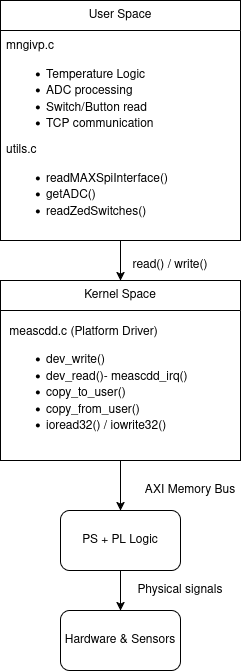
\includegraphics[width=0.25\textwidth]{media/h2peta1.png}
    \caption{Complete Architecture Diagram}
    \label{fig:meascddArch}
\end{figure}


\subsubsection{Stateful Communication via REGNUM\_ID}
A unique architectural feature of this system is the use of a "control ID" to manage the state of the communication channel. The driver uses a reserved constant, \texttt{REGNUM\_ID (0x0FF)}, to distinguish between a command to write data to the hardware and a command to select a register for future observation.

When the user-space program writes a \texttt{MeasObj\_struct} with rnum set to \texttt{0x0FF}, the driver does not toggle any hardware pins; instead, it updates an internal kernel variable named \texttt{Reg\_Num}. This variable then dictates which hardware register will be accessed during the subsequent read() system call. This design allows the user-space program to "poll" different hardware registers (such as status vs. data registers) using a single, unified file descriptor.

\subsection{Critical Section Management and LED Bitmasking}
The driver manages a shared hardware resource: the LED and status register (Register 0). In this system, Register 0 is modified by two different entities: the user-space application (to set status LEDs) and the Kernel's Interrupt Service Routine (to toggle a "heartbeat" LED).

To prevent these two entities from overwriting each other, the dev\_write function employs bitmasking logic. When a user writes to Register 0, the driver preserves the 7th bit (the interrupt-controlled LED) while updating the lower 7 bits with user data. This ensures that the visual "heartbeat" maintained by the meascdd\_irq routine remains consistent even when the user application is actively changing the state of other LEDs.

\subsection{Interrupt Service Routine and Timing}
The hardware is designed to generate periodic interrupts based on a 100ms timer. The driver defines this timing constant as 0x009896ff. Upon receiving an interrupt signal, the \texttt{meascdd\_irq} routine is executed by the kernel.
The ISR follows a precise "Acknowledge and Re-arm" sequence:
\begin{itemize}
\item Acknowledgment: It writes the MBINT\_ACKN flag to the control register to clear the hardware interrupt line.
\item Action: It toggles the 7th bit of the Led\_Output variable using a XOR operation \texttt{(\^\ = 0x080)} to create the blinking effect.
\item Re-arming: It writes back the MBINT\_ENABLE flag along with the timer constant to ensure the next interrupt occurs in exactly 100ms.
\end{itemize}

\subsection{Application Integration: Temperature Sensing Logic}
The system's primary utility is demonstrated in the TempMeasure function, which interfaces with a MAX31865 RTD-to-Digital converter. The user-space program uses the driver to "bit-bang" configuration data into the device.
For example, the application sends the hex value 0x81 to initialize the PMB1 hardware and 0xA1 to trigger a single-shot temperature conversion. The driver facilitates this by wrapping these hex commands into MeasObj\_struct objects, which are then transmitted across the kernel boundary to the physical SPI-over-AXI bridge. The application then calculates the final temperature using the formula T=xadc×0.03125−256.0, where xadc is the raw data retrieved via the driver from registers 1 and 2.

\subsection{Driver Registration and Probe Execution}
The seamless integration fo the meascdd module into the Linux kernel is governed by the Platform Driver framework, which automates hardware discovery through the device tree. Rather than manually searching for hardware, the kernel uses a matching mechanism to link the driver code to the physical AXI IP core defined in the system’s firmware. 

\begin{minted}[tabsize=4, breaklines, bgcolor=lightgray]{c}
static struct platform_driver meascdd_driver = {
    .probe = meascdd_probe,
    .remove = meascdd_remove,
    .driver = {
    .name = "meascdd",
    .of_match_table = meascdd_of_match,
    },
};
\end{minted}

The \texttt{platform\_driver} structure formally registers the \texttt{meascdd} driver with the Linux kernel’s platform driver framework. This structure defines the lifecycle callbacks and matching configuration required for driver binding.

Key elements:
\begin{itemize}
    \item \texttt{.probe}: Points to \texttt{meascdd\_probe()}, which is executed when the kernel finds a matching device tree node
    \item \texttt{.remove}: Points to \texttt{meascdd\_remove()}, which is called when the driver is unloaded or the device is removed.
    \item \texttt{.name}: Logical driver name used internally by the kernel.
    \item \texttt{.of\_match\_table}: Links the driver to the Open Firmware matching table (\texttt{meascdd\_of\_match}). This enables automatic binding when the kernel parses a Device Tree node containing: “xlnx, measdif-1.0” compatible string.
\end{itemize}

During kernel boot or module insertion, the Device Tree Blob (DTB) is parsed. When a node with \texttt{compatible = "xlnx,measdif-1.0"} is detected, the platform driver framework invokes \texttt{meascdd\_probe()}.



\subsubsection{Device Tree parsing and probe execution}
During the kernel's boot or module insertion phase, the system parses the Device Tree Blob (DTB) to identify available hardware. The kernel specifically looks for a node containing the property compatible = "xlnx,measdif-1.0". This string acts as a unique hardware identifier. The meascdd.c module contains an of\_match\_table that explicitly lists this string, signaling to the kernel that this specific driver is capable of managing that hardware instance.

\subsubsection{The Probe Sequence}
Once a match is confirmed, the kernel triggers the meascdd\_probe function, which serves as the "constructor" for the device. This function is responsible for several critical setup tasks:
\begin{itemize}
\item Resource discovery: The driver calls platform\_get\_resource to retrieve the physical base address and the Interrupt Request (IRQ) number assigned to the hardware in the Device Tree.
\item Memory locking: It invokes request\_mem\_region to ensure no other driver can claim the physical memory space assigned to the PMB1 registers.
\item I/O Mapping: The physical address is converted into a kernel-accessible virtual address via ioremap, which is then stored in the global Meas\_Base\_Address pointer for use by the read and write functions.
\end{itemize}

\subsubsection{Character Device Creation}
Beyond hardware initialization, the probe function establishes the user-space interface. It dynamically allocates a major number using register\_chrdev and creates a device class in sysfs. This sequence culminates in the creation of the /dev/meascdd node, effectively bridging the gap between the kernel's internal hardware representation and the standard Linux filesystem.


\subsubsection{Interrupt Attachment}
The final stage of the probe execution involves the request\_irq function. The driver registers the meascdd\_irq routine as the handler for the device's hardware interrupt. By doing so, the driver tells the kernel exactly which code to execute whenever the hardware timer—defined by the TIMER100ms constant—reaches its terminal count. This registration allows the driver to toggle the LED "heartbeat" without requiring any active processing from the user-space application.

\section{System execution Sequence diagram}
\subsection{Boot and Driver Binding}
\begin{figure}[H]
    \centering
    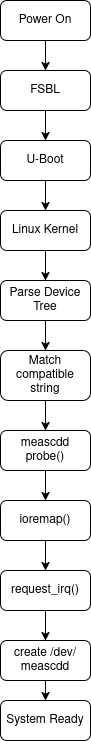
\includegraphics[scale = 0.7]{media/h2peta2.png}
    \caption{Boot and Driver Binding Architecture}
    \label{fig:bootAndDriverBinding}
\end{figure}

\subsection{Register write transition}
This architecture diagram demonstrates the sequence of starting ADC.

\begin{figure}[H]
    \centering
    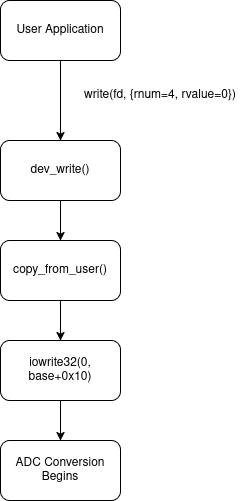
\includegraphics[scale = 0.6]{media/h2peta3.png}
    \caption{Register write transition Architecture}
    \label{fig:registerWriteTransition}
\end{figure}

\subsection{Register read transition}
\begin{figure}[H]
    \centering
    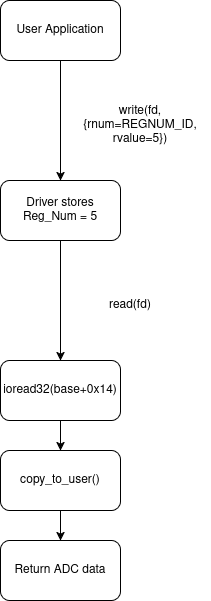
\includegraphics[scale = 0.6]{media/h2peta4.png}
    \caption{Register read transition Architecture}
    \label{fig:registerReadTransition}
\end{figure}


\subsection{Building the Image}
After integrating the custom kernel module (meascdd.c) and user-space application (mngivp.c) are integrated into the project environment, the next step is building the system image. 

The image is built using the petalinux command 
\begin{minted}[tabsize=4, breaklines, bgcolor=lightgray]{text}
petalinux-build
\end{minted}

Unlike compiling a standalone C program, this command invokes the Yocto-based build system to generate an entire bootable Linux software stack tailored for the target Zynq-7000 platform.

\subsubsection{PetaLinux Build Stages}
Each stage of image build process is given below
\begin{itemize}
\item Kernel compilation (inlcuding LKM)
\item Device Tree configuration
\item RootFS generation
\item FIT image packaging
\end{itemize}




\subsubsection{Component Integration}
The final output of this process is typically the image.ub file, which is a FIT (Flattened Image Tree) format. This single file acts as a container for several critical components:

\begin{itemize}
\item \textbf{The Kernel Image:} The core operating system that manages system resources and schedules tasks.
\item \textbf{The Root Filesystem (RootFS)}: The environment where the mngivp application resides and where the character device node is created.
\item \textbf{The Device Tree Blob (DTB)}: The binary map that tells the driver exactly where the PMB1 hardware registers are located in memory.
\end{itemize}

\subsubsection{Deployment and Integration}
Once the build is complete, the image.ub and the bootloader (BOOT.BIN) are copied to the SD card. Upon power-up:
\begin{itemize}
\item The kernel parses the device tree and matches the "compatible" string to the meascdd driver.
\item The probe function executes, remapping the hardware registers and registering the major number.
\item The user executes ./mngivp, which opens /dev/meascdd to begin temperature or ADC acquisition.
\end{itemize}

\subsubsection{Verification of the Build}
A successful build can be verified by checking the /lib/modules/ directory on the target rootfs for the meascdd.ko file or by running ls /dev/meascdd once the system has booted. If the build was successful, the hardware heartbeat LED managed by meascdd\_irq should begin toggling at 100ms intervals as soon as the driver is loaded.

\subsection{Runtime Verification}
The final step involved is to verify that the integration performed during the build process correctly translates into functional hardware-software communication on the physical board.
After booting the board, the following were verified:
\begin{itemize}
\item Driver loaded: This command lists all currently loaded kernel modules. Seeing meascdd in this list confirms that the kernel successfully matched the "compatible" string from the Device Tree with the driver's of\_match\_table and executed the module's initialization code.
\item Device node exists: The presence of this file confirms that the major number was successfully registered and that the meascdd\_probe function completed its character device registration sequence without error.
\item dmesg logs: This allows for the inspection of specific printk and dev\_info messages generated during the driver's execution.
\end{itemize}
Based on the logs and system state, the following critical milestones were reached:
\begin{itemize}
\item AXI Base Address Mapped: The log confirms that platform\_get\_resource successfully retrieved the physical memory address from the Device Tree and that ioremap successfully mapped it to a kernel-accessible virtual address (stored in Meas\_Base\_Address).
\item Interrupt Registered: The verification confirms that request\_irq was successful for the IRQ number specified in the Device Tree. This is often visually confirmed by the 100ms LED "heartbeat" toggled by the meascdd\_irq routine.
\item Device Successfully Initialized: The "MEAScdd: registered correctly" and "MEAScdd: initialized" messages confirm that the major number was allocated and the platform driver is ready to handle read() and write() calls from the mngivp.c application.
\end{itemize}


\subsection{Summary}
The PetaLinux integration establishes a complete hardware–software abstraction layer between the AXI-based measurement IP and the user-space application. The Vivado hardware design is exported as an XSA file and imported into PetaLinux, enabling automatic generation of the device tree and kernel configuration aligned with the Zynq-7000 architecture.

The custom meascdd driver is implemented as a Linux platform driver and bound to the hardware instance using Open Firmware device tree matching. Upon successful compatible string matching, the kernel invokes the \texttt{probe()} function, which performs resource discovery, physical memory mapping using \texttt{ioremap()}, interrupt registration via \texttt{request\_irq()}, and character device creation.

User-space communication is achieved through a structured interface (\texttt{MeasObj\_struct}) using \texttt{copy\_from\_user()} and \texttt{copy\_to\_user()} mechanisms. Register addressing follows a strict 32-bit word-aligned mapping scheme to ensure AXI compliance. A stateful register selection mechanism using \texttt{REGNUM\_ID} enables efficient multi-register access over a single character device interface.

Periodic hardware interrupts are handled by the \texttt{meascdd\_irq} ISR, which acknowledges the interrupt, updates system state, and re-arms the timer to maintain deterministic 100 ms execution cycles.

The complete system image is generated using the Yocto-based PetaLinux build system, producing a bootable FIT image (\texttt{image.ub}) containing the Linux kernel, device tree, and root filesystem. Runtime verification confirms correct driver binding, memory mapping, interrupt servicing, and character device initialization.
This architecture ensures secure, structured, and deterministic communication between FPGA-based AXI hardware and high-level user applications within a Linux environment.
